%%%%%%%%%%%%%%%%%%%%%%%%%%%%%%%%%%%%%%%%%%%%%%%%%%%%%%%%%%%%%%%%%%%%%%%%%%
% Signals of U2 and i1 and i2
%%%%%%%%%%%%%%%%%%%%%%%%%%%%%%%%%%%%%%%%%%%%%%%%%%%%%%%%%%%%%%%%%%%%%%%%%%
\begin{solutionfigure}[htb]

 %   \documentclass{standalone}
 %   \usepackage{pgfplots}
 %   \pgfplotsset{compat=1.18} % Kompatibilität für neuere Versionen
        \centering
        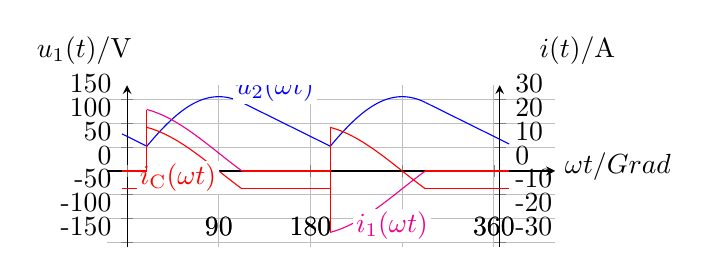
\begin{tikzpicture}
            \begin{axis}[
                    % x/y range adjustment
                    xmin=-20, xmax=420,
                    ymin=-160, ymax=180,
                    samples=500,
                    axis y line=center,
                    axis x line=middle,
                    extra y ticks=0,
                    % Label text
                    xlabel={$\omega t / \text{Grad}$},,
                    ylabel={$u_\mathrm{1}(t)/\mathrm{V}$},
                    % Label adjustment
                    x label style={at={(axis description cs:1,0.5)},anchor=west},
                    y label style={at={(axis description cs:-.05,.97)},anchor=south,yshift=0.2cm},
                    width=0.6\textwidth,
                    height=0.3\textwidth,
                    % x-Ticks
                    xtick={0,90,180,270,360},
                    xticklabels={,90,180,270,360},
                    xticklabel style = {anchor=north,yshift=-0.4cm},
                    % y-Ticks
                    ytick={150,100,50,-50,-100,-150},
                    yticklabels={150,100,50,-50,-100,-150},
                    yticklabel style = {yshift=0.2cm,anchor=east},
                    % Grid layout
                    grid,
                    %grid style={line width=.1pt, draw=gray!10},
                    %major grid style={line width=.2pt,draw=gray!90},
                ]
                % Voltage u2(wt) if supplied by u1(wt)
                \addplot[blue, domain= 19.3:112.8] {abs(156*sin(x))};                
                \addplot[blue, domain= 199.3:292.8] {abs(156*sin(x))};                
                % Voltage u2(wt) if supplied by uc(wt)
                \addplot[blue, domain=-5:19.3] {143.8-(x+67.2)*1.06};                
                \addplot[blue, domain=112.8:199.3] {143.8-(x-112.8)*1.06};                
                \addplot[blue, domain=292.8:375] {143.8-(x-292.8)*1.06};                
                % Label of u1
                \node[blue, fill=white, inner sep = 1pt, anchor = south] at (axis cs:145,140) {$u_{\mathrm{2}}(\omega t)$};

            \end{axis}     
            \begin{axis}[
                % x/y range adjustment
                xmin=-20, xmax=420,
                ymin=-32, ymax=36,
                samples=500,
                axis y line=right,
                axis y line shift=-20pt,
                axis x line=middle,
                extra y ticks=0,
                % Label text
                ylabel={$i(t)/\mathrm{A}$},
                % Label adjustment
                y label style={at={(axis description cs:1.05,.97)},anchor=south, rotate=270,yshift=0.2cm},
                width=0.6\textwidth,
                height=0.3\textwidth,
                % x-Ticks
                xtick={0,90,180,270,360},
                xticklabels={,90,180,270,360},
                xticklabel style = {anchor=north,yshift=-0.4cm},
            % y-Ticks
                ytick={30,20,10,-10,-20,-30},
                yticklabels={30,20,10,-10,-20,-30},
                yticklabel style = {yshift=0.2cm,anchor=west},
                % Grid layout
                % grid=both,
                % grid style={line width=.1pt, draw=gray!10},
                % major grid style={line width=.2pt,draw=gray!90},
            ]
                % Current ic(t)
                \addplot[red, domain= 19.3:112.8] {19.4*cos(x)};                
                \addplot[red, domain= 199.3:292.8] {-19.4*cos(x)};                
                % Current ic(t) if supplied by uc(t)
                \addplot[color=red,mark=none,solid] coordinates{
                    (-5, -7.5)
                    (19.3, -7.5)
                    (19.3,18.3)
                    }; 
                \addplot[color=red,mark=none,solid] coordinates{
                    (112.8, -7.5)
                    (199.3, -7.5)
                    (199.3,18.3)
                    }; 
                \addplot[color=red,mark=none,solid] coordinates{
                    (292.8, -7.5)
                    (375, -7.5)
                     }; 
                % Label of ic
                \node[red, fill=white, inner sep = 1pt, anchor = south] at (axis cs:50,-10) {$i_{\mathrm{C}}(\omega t)$};

                % Current i1(wt)
                \addplot[magenta, domain= 19.3:112.8] {19.4*cos(x)+7.5};                
                \addplot[magenta, domain= 199.3:292.8] {19.4*cos(x)-7.5};                
                % Current i1(wt) if supplied by uc(t)
                \addplot[color=red,mark=none,solid] coordinates{
                    (-5,0)
                    (19.3,0)
                    (19.3,25.8)
                    }; 
                \addplot[color=red,mark=none,solid] coordinates{
                    (112.8,0)                    
                    (112.8,0)
                    (199.3,0)
                    (199.3,-25.8)
                    }; 
                \addplot[color=red,mark=none,solid] coordinates{
                    (292.8,0)                    
                    (292.8,0)
                    (375,0)
                    }; 
                % Label of i1
                \node[magenta, fill=white, inner sep = 1pt, anchor = south] at (axis cs:260,-30) {$i_{\mathrm{1}}(\omega t)$};
            \end{axis}
        \end{tikzpicture}
        \caption{Voltage at primary side.}
        \label{sfig:ex05_Voltage_u2_andCurrent_i1_ic}
\end{solutionfigure}